\documentclass[]{article}
%\documentclass[conference,final]{IEEEtran}


% Use utf-8 encoding for foreign characters
\usepackage[utf8]{inputenc}

% Setup for fullpage use
\usepackage{fullpage}

% Uncomment some of the following if you use the features
%
% Running Headers and footers
%\usepackage{fancyhdr}

% Multipart figures
%\usepackage{subfigure}

% More symbols
%\usepackage{amsmath}
%\usepackage{amssymb}
%\usepackage{latexsym}

% Surround parts of graphics with box
\usepackage{boxedminipage}

% Package for including code in the document
\usepackage{listings}

% If you want to generate a toc for each chapter (use with book)
\usepackage{minitoc}

% This is now the recommended way for checking for PDFLaTeX:
\usepackage{ifpdf}

\usepackage{url}

\usepackage{enumerate}
\usepackage{subfigure}

%\newif\ifpdf
%\ifx\pdfoutput\undefined
%\pdffalse % we are not running PDFLaTeX
%\else
%\pdfoutput=1 % we are running PDFLaTeX
%\pdftrue
%\fi

\ifpdf
\usepackage[pdftex]{graphicx}
\else
\usepackage{graphicx}
\fi

\usepackage{color}
\definecolor{listinggray}{gray}{0.95}
\definecolor{darkgray}{gray}{0.7}
\definecolor{commentgreen}{rgb}{0, 0.4, 0}
\definecolor{darkblue}{rgb}{0, 0, 0.4}
\definecolor{middleblue}{rgb}{0, 0, 0.7}
\definecolor{darkred}{rgb}{0.4, 0, 0}
\definecolor{brown}{rgb}{0.5, 0.5, 0}

\newif\ifdraft
\drafttrue
\ifdraft
\newcommand{\jhanote}[1]{ {\textcolor{red} { ***shantenu: #1 }}}
\newcommand{\alnote}[1]{ {\textcolor{blue} { ***andre: #1 }}}
\newcommand{\smnote}[1]{ {\textcolor{green} { ***sharath: #1 }}}
\newcommand{\msnote}[1]{ {\textcolor{cyan} { ***mark: #1 }}}
\else
\newcommand{\alnote}[1]{}
\newcommand{\athotanote}[1]{}
\newcommand{\smnote}[1]{}
\fi


%\title{BigJob, ManyJob, Pilot-Store, ... -- Abstractions for dynamic ...}

\title{TROY: Towards Dynamical Distributed Applications}


\author{  }

%\date{}


\begin{document}

\ifpdf
\DeclareGraphicsExtensions{.pdf, .jpg, .tif}
\else
\DeclareGraphicsExtensions{.eps, .jpg}
\fi

\maketitle

\jhanote{Alternate title: The Tiered Resource OverlaY framework
  (TROY): An Empirical Framework for Pilot-* Abstractions}


\begin{abstract}

\end{abstract}

\section{Introduction}
\subsection{Aims of the paper}
\begin{itemize}

\item Establish the need for dynamic execution of applications -
  distributed as well as high-end performance.

\item We define the basic characteristics of the dynamic apps and we
  understand the requirements of dynamic apps need to do in a
  distributed environment.

\item We understand the capability that must be provided by the
  infrastructure to support these application

\item We describe the pilot-job as a good prototype of an abstraction
  that supports dynamic execution

\item We define the characteristics that need to be supported by a
  pilot-job \jhanote{Infrastructure or Application
    characteristics?} \alnote{I think we meant application characteristics}

\item An extensible framework to aid an understanding of pilot-jobs
  and the ability to compare, contrast and understand different
  pilot-jobs.

%Basic minimal model for the different kinds of pilot-jobs

\item Empirical implementation of TRoY and demonstration of
  concurrent/interoperation between equivalent but distinct Pilot-Job
  implementation 

% Examples of distinct pilot-jobs from SAGA world  

\end{itemize}

\subsection{Motivation}

Distributed systems are inherently dynamic: resources can suddenly fail or 
new resources can become available at any time. Generally there are two types
of dynamism.
\begin{itemize}
    \item \textbf{Resource dynamism:} Distributed systems are inherently dynamic
     -- resources can become available or fail at any time. The same holds for
      network connections. Further, hybrid infrastructures comprised of 
      different resources classes can vary significantly in their costs for 
      usage, performance, availability and the guarantees for quality of service 
      they provide.
      
	\item \textbf{Application dynamism} describes the requirement of many
applications to support dynamic resource requirements. An example are
applications whose execution time resource requirements cannot be determined
exactly in advance (either due to changes in runtime requirements) or those that
are dependent on dynamic data (e. g. sensor, in-transit or variable source/sink
of data). Further, the application requirements may change, due to,
for example, a failure or an application event.
\end{itemize}

Further things to consider:
\begin{itemize}
    \item dynamic scheduling
    \item dynamic task placement
    \item autonomic behaviors: Monitoring of the system/application state and 
    adaptations of the application and/or resources to respond to changing 
    requirements or environment.
\end{itemize}

The real power of distributed systems, however, arises from adaptive algorithms
and implementations that provide applications with an agile execution model, and
thus the ability to use resources dynamically as opposed to a static execution
model inherited from parallel and cluster computing

\msnote{What paper is this referring to? I disagree btw, the real power does not arise from adaptive algorithms and implementations, instead, the power can only be fully exploited by using those.}\alnote{\url{http://www.cct.lsu.edu/~sjha/select_publications/adaptive_repex_ptrsa.pdf}}

\section{Pilot-* : An abstraction for Dynamic Execution}

The uptake of distributed infrastructures by scientific applications
has been limited by the availability of extensible, pervasive and
simple-to-use abstractions which are required at multiple levels –
development, deployment and execution stages of scientific
applications. The Pilot-Job abstraction has been shown to be an
effective abstraction to address many requirements of scientific
applications. Specifically, Pilot-Jobs support the decoupling of
workload submission from resource assignment; this results in a
flexible execution model, which in turn enables the distributed
scale-out of applications on multiple and possibly heterogeneous
resources. Most Pilot-Job implementations however, are tied to a
specific infrastructure. In this paper, we describe the design and
implementation of a SAGA-based Pilot-Job, which supports a wide range
of application types, and is usable over a broad range of
infrastructures, i.e., it is general-purpose and extensible, and as we
will argue is also interoperable with Clouds.

\msnote{regarding SAGA-based, is it really SAGA based, or rather an
  extension?}\alnote{The implementation utilizes SAGA, but it is not a
  really a SAGA extension yet - there is not even a draft for a spec
  extension yet}

\msnote{why the explicit mentioning of clouds while in the same sentence there is referred to a "broad range of infrastructures"}

\subsection{Model:}

We propose a set of fundamental properties/characteristics that can be
used to construct a framework to describe pilot-*..

\begin{itemize}
	\item \textbf{Task binding:~\cite{diane-thesis}} 
		\begin{itemize}
			\item In the traditional early binding approach a job carries
			 exactly one task which is specified at a time of job submission.
			\item Late binding is a scheduling and coordination
			 method, where work is assigned to a job at runtime rather than at
			 submission time.
			\begin{itemize}
				\item At sub-job submission 
				\item After sub-job submission
			\end{itemize}
		\end{itemize} 	

	\item \textbf{Resource Types:}
	\begin{itemize}
		\item Cluster support, i.e. Number of resources per BigJob
		\item Number of concurrent sub-jobs per BigJob agent
	\end{itemize}
	\item \textbf{Coordination} describes how the various components of 
	the Pilot-Job framework are	coordinated. Possible values for this vector include data
	flow, control flow, SPMD (where the control flow is implicit in all copies of the single program), master-worker
	(the work done by the workers is controlled by the master),
	\begin{itemize}
		\item The data flow describes the flow of messages between the components of the framework, e.\,g.\ point-to-point messaging or publish-subscribe (see Communication).
		\item The control flow describes how the various components of the
		 framework are managed. In the context of pilot-jobs this particularly means how the resource on which a sub-job is executed is determined. Generally, it can be differentiated between the two kinds of decision makings:
			\begin{itemize}
				\item Central: Decisions are centrally made by a master
				 process, i.\,e.\ a central manager decides which sub-job is
				 executed on what resource.
				\item Decentral: Control is distributed among the 
				different components. Pilot-Jobs with decentralized decision 
				making often utilize agents that accepts respectively pull 
				sub-jobs according to a set of defined criteria.
			\end{itemize}
			
			\begin{tabular}{|l|c|c|}
				\hline
				&central &decentral\\
				\hline
			Simplicity  &++			&o \\ \hline
			Decision Quality &+ 	&++ \\ \hline
			Flexibility &+			&++ \\ \hline
			Adaptivity  &+ 			&++ \\ \hline
			Failure Resilience &+   &++\\ \hline
			
			\end{tabular}
		% \item Sub-Job pull vs. push applies to control and data flow (different objects that are pushed/pulled)

	\end{itemize}	
	\item \textbf{Communication:} Data can be exchanged by messages
(point-to-point, all-to-all, one-to-all, all-to-one, or group-to-group),
stream (potentially unicast or multicast), publish/subscribe or through shared
data.
	\begin{itemize}
		\item Remote procedure calls: CORBA, RMI
		\item Messaging: point-to-point, collective operations
		\item Shared data space (e.\,g.\ tuple space): BigJob e.g. uses the Advert service to share data between the manager and the agent (such as task information). In general, this is associated with a push/pull coordination schema, i.e. the manager pushes something to the shared data space and the agents periodically check for new data.
	\end{itemize} 
	\item \textbf{Dynamic Resources:}
		\begin{itemize}
			\item Push/Pull model for growing/shrinking resources
			\item How is this decision made?
		\end{itemize}
	\item \textbf{Data management:} Managing input and output files can be critical in particular with the current increase of data volumes. Pilot-Jobs can support different kinds of data management, e.\,g.\ file stage-in and out. Also, it can provide integration with other kinds of data systems.
	\item \textbf{Fault tolerance:} Large, distributed Grids are highly dynamic and inherently prone to failures and thus unreliable. To deal with failures, systems can deploy strategies, such as automatic resubmission etc.
	\item \textbf{Resource abstraction:} SAGA vs. GANGA
	\msnote{Whats this comparison aiming at?} \alnote{This is not a really 
	defining characteristic. But, since we are talking about abstractions, I 
	thought it might be useful to describe how resources are accessed.}
	\item \textbf{End-user abstraction:} BigJob API
	\item Task scheduling and prioritization
	\begin{itemize}
	 			\item Policies and Algorithms
	 			\item What attributes are required?
	 			\item Multi-level scheduling
	 			\item Integration of data- and compute scheduling
	 			\item see MLS paper
	\end{itemize}
	\item \textbf{Agent:} Does every pilot-job implementation have an agent? What are the tasks of an agent?
	\begin{itemize}
	    \item Wikipedia Definition: may refer to one who acts for, or in the place of, another, by authority from him; one entrusted with the business of another.
	    \item \textbf{Tasks of an agent:}
	    \begin{itemize}
	        \item manages control flow
	        \item mapping tasks to resources
	        \item resource management
	        \item coordination between different components
	        \item state management of the complete pilot job state
	        \item discovering local information
        \end{itemize}


     \item \textbf{Distribution of agent / Agent Hierarchies} (we could introduce a resource agent or sub-agent):
        \begin{itemize}
    	    \item No distribution: BigJob-Cloud -- direct dispatching of sub-jobs from manager (agent is component of manager)
            \item Lightweight resource agent: Diane -- Agent on resource is used as a dispatcher (capacity = 1 sub-job)
            \item Heavy resource agent: SAGA BigJob -- resource management, sub-job dispatching, state management...
    \end{itemize}

	\item How many resources are managed by an agent (BigJob Agent vs. Diane Worker Agent)? How many tasks can be assigned to a agent? Single core worker, partial node worker, whole node worker, multi node worker (BigJob
default). This characteristic influences: 
    \begin{itemize}
        \item Scalability
        \item Scheduling possibilites
        \item Fault tolerance
    \end{itemize}
    \end{itemize}
	\item Supported middleware types and infrastructures	
	\item Security
	\item \textbf{Push vs Pull} We define the terms push and pull based upon the determinism of the binding. If the task is centrally explicitly addressed to a specific pilot, and there is thus no freedom for a pilot to select the task, we speak of a push model. In all other situations, when there is a degree of freedom for the pilots to select a task, we speak of pull.
	
	
	

	
	
\end{itemize}

\alnote{Comments from call (24/04/2011):
\begin{itemize}
	\item Decision on the resources where the BigJob is submitted to
	\item HTC it is quite common that you no knowledge about resources
	\item push/pull for task not for agent
	\item ManyJob: agent being pushed, task being pulled (agent notify master when active)
	\item Marc: Data intensive also become more memory intensive - decoupling of core and worker needed
	\item Further defining task binding: late binding vs. early vs. partial binding	
	\item Sharath: Establish cloud vs. grid BigJob
	\item Affinity does not arise in the static BigJob - should remain just in dynamic
	\item Multiple BigJob instead of ManyJob?
\end{itemize}
Call (27/04/2011)
\begin{itemize}
	\item module for adaptive data, adaptive scheduling    
\end{itemize}
}


\subsection{Definitions}

\jhanote{I propose this be after characteristics -- as the
  characteristics are fundamental and this is an 'abstract
  framework' to support the characteristics}

\jhanote{I also propose we equate task==workload wherein the task is
  independent of any resource}

\begin{enumerate}[A.]
	
	
	\item\textbf{Pilot-Agent / Agent / Pilot-Job / Worker / Placeholder Job / 
	Resource Agent / Placeholder-Job:} A PJ is a container for multiple \textbf{tasks/jobs?} 
	that may be dynamically added to it. Tasks are ultimately loaded onto 
	specific resources via late-binding. In other words, PJ provides a mechanism 
	to decouple “task coordination” from “resource mapping”. Facilities provided 
	include the creation of a PJ, insertion of tasks, and attachment to a CPU 
	resource pool for late-binding task execution. \alnote{ the "thing" that is sent out to \ref{resource}} \label{pilot-agent}    
	
	\begin{itemize}
	   	\item Big-Job Agent: capacity (physical size) is a property of an agent. 
    	cardinality: how many sub-jobs can be managed by an agent?
    	\item Sub-Job Agent: Agent assignment should be separated from resource 
    	assignment. Agent has the freedom to assign tasks to sub-job in any way 
    	it want. Agent can do local decisions.    
	\end{itemize}
	\item \textbf{Task:} A task is a workload that is independent form a 
	resource. A task can be assigned to a sub-job/job.
	\item \textbf{Sub-Job/Job:} Sub-jobs are schedule-able units and are the 
	unit of works that are sent down to \ref{pilot-agent} to be executed. 
	Sub-jobs/jobs are used to reserve the resources required by a task. A 
	sub-job runs an instance of \ref{application-program}. 	
	\item \textbf{Task Scheduler:} A task scheduler is the the unit responsible for mapping tasks 
	to resources and thus, creating jobs. 	
	\item \textbf{BigJob:} The entity that is presented to 
	\ref{application-program} or 2. The entity that gets scheduled on 
	\ref{resource}.	
	\item \textbf{Resource:} A storage/compute Resource that has a common entry 
	point (like a queue) \label{resource}
	\item \textbf{Headnode:} entity that is the entrance for an \ref{resource}
	\item \textbf{Master / Manager / Central / Control / Coordination:} 
	something central
	\item \textbf{Application:} is upper layer on the stack e.g. DARE-NGS. The application utilizes the BigJob API to execute instances of \ref{application-program}. \label{application}
	\item \textbf{Program / Executable / Software / Application Kernel:} An application kernel is actual binary that gets run, e.g. \texttt{/usr/local/bin/bfast}. \label{application-program}	
\end{enumerate}




\begin{figure}[htbp]
        \centering
    \subfigure{
\includegraphics[width=0.4\textwidth]{figures/task-job1.pdf}}\qquad\qquad
    \subfigure{
\includegraphics[width=0.4\textwidth]{figures/task-job2.pdf}}        
    \caption{Relationship between Task and Sub-Job/Job}
    \label{fig:figures_task-job1}
\end{figure}    



\textbf{Diane Definition of Terms: } The computation consists of many worker
processes which communicate with one master process (the worker processes do not
need to share the filesystem nor memory). The ensemble of computation is called
a run and it consists of many tasks which may be executed in parallel. A task is
defined as a set of parameters which are produced by the RunMaster (running on a
master node) and consumed by the WorkerAgent (running on a worker node).



\section{PilotJob Implementations}

Table~\ref{tab:pilotjob_overview} gives an overview of different pilot-job
implementations and their characteristics. BigJob currently supports different
Backends: SAGA BigJob can be used in conjunction with different SAGA adaptors,
e.\,g.\ the Globus, PBS, Amazon Web Service and local adaptor. In addition to
the SAGA-based reference implementation, there are various other implementations
of the BigJob API, e.\,g.\ for Amazon Web Services, Azure and Condor resources.

% \begin{itemize}
%     \item SAGA/Grid: Globus, PBS, Local, 
%     \item EC2-style Clouds (FutureGrid, EC2, Eucalyptus)
%     \item Azure
%     \item Condor
%     \item Diane
% \end{itemize}

\msnote{Glide-In I assume, and not normal condor?}\alnote{yes}

\begin{table}[t]
\begin{tabular}{|l|p{2.5cm}|p{2cm}|p{2cm}|p{2cm}|p{2cm}|}
	\hline
	&\textbf{Task Binding} &\textbf{Cluster Support} &\textbf{Coordina\-tion} & \textbf{Communica\-tion} &\textbf{Dynamic Resources}\\
	\hline
	\textbf{BigJob} & &&&&\\
	\hline
	SAGA BigJob & &&&&\\
	\hline
	\hspace{4mm} Globus/PBS adaptor  &late binding (at sub-job submission)  
									 &yes &central decision making &SAGA Advert (pull/push) &no\\  
	\hline
	\hspace{4mm} Cloud adaptor (EC2) &late binding (at sub-job submission)  
									 &no &central decision making &SAGA Advert (pull/push) &no\\ 
    \hline
   BigJob-Condor &late binding (after sub-job submission by Condor) &yes &central decision making &Condor-internal &no\\
	\hline
 	BigJob-Cloud &late binding (at sub-job submission) &yes &central decision making 
				 &local python-based queue / SAGA Job (SSH adaptor) &no\\ 
	\hline
	BigJob-Azure &late binding (at sub-job submission)
	             &no &central decision making &Azure Storage (push/pull) &no\\ 
	\hline
    BigJob-Diane &late binding  &yes &decentral decision making &CORBA (pull from master) &yes\\ 
	\hline	
	\textbf{Dynamic BigJob} & &&&&\\
	\hline
    Dynamic BigJob &late binding (after job submission) &same as BJ &central decision making &same as BJ &(yes in future)\\
    \hline
    %   ManyJob-Cloud &late binding (after job submission) &no &central decision making &SAGA Job (SSH) (push) &no\\
    % \hline 
    % ManyJob-Affinity &late binding (after job submission)
    % &yes &central decision making &SAGA Advert (push/pull) &no\\
    % \hline
\end{tabular}
\caption{Characteristics of Pilot-Job Implementations According 
		to Defined Vectors} \label{tab:pilotjob_overview}
\end{table}		



\subsection{SAGA BigJob}

%\begin{figure}[t]
%    \centering
%        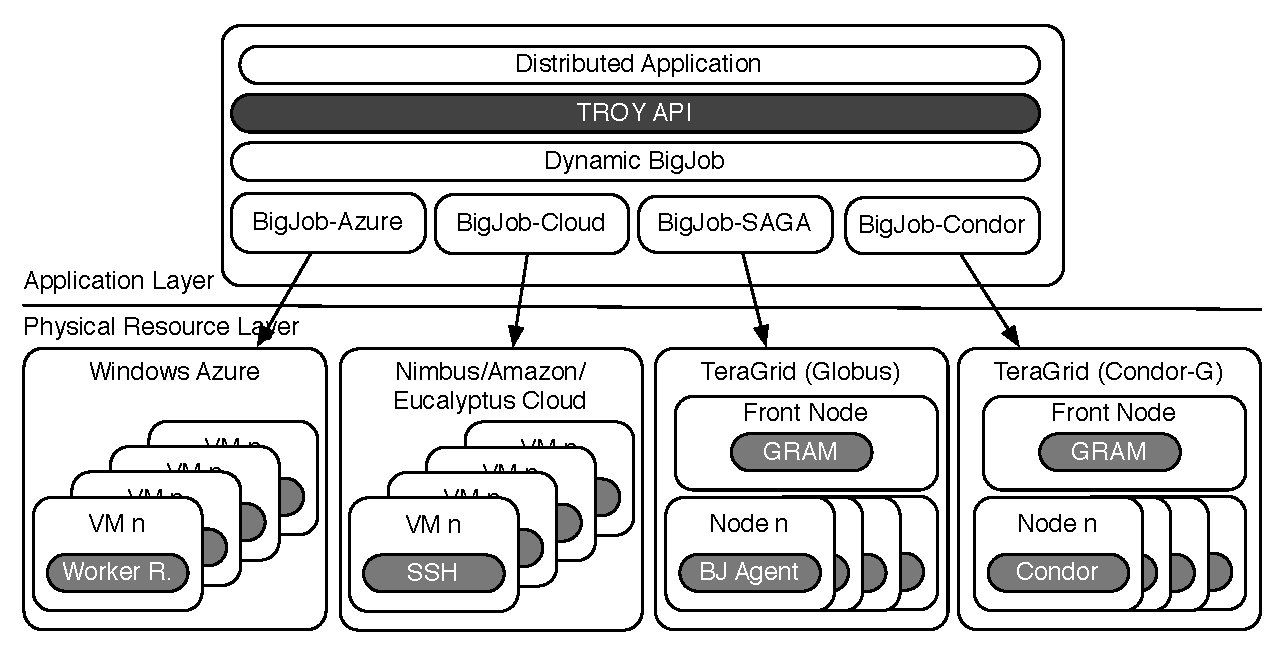
\includegraphics[width=0.7\textwidth]{figures/distributed_pilot_job.pdf}
%    \caption{BigJob API and Implementation}
%    \label{fig:figures_distributed_pilot_job}
%\end{figure}

BigJob comprises of an API (see Figure~\ref{fig:figures_distributed_pilot_job}
and section~\ref{sec:api}) and various resource-specific implementations of the
API. The SAGA-based Pilot-Job is the reference implementation of the BigJob API.
It supports a wide range of application types, and is usable over a broad range
of infrastructures, i.\,e.\ it is general-purpose and extensible.


\subsection{BigJob for Cloud Computing}

At the execution level, clouds differ from Clusters/Grids in at least a couple
of different ways. In cloud environments, user-level jobs are not typically
exposed to a scheduling system; a user-level job consists of requesting the
instantiation of a virtual machine (VM). Virtual machines are either assigned to
the user or not (this is an important attribute that provides the illusion of
infinite resources). The assignment of job to a VM must be done by the user (or
a middleware layer as BigJob). In contrast, user-level jobs on grids and 
clusters are exposed to a scheduling system and are
assigned to execute at a later stage. Also a description of a grid job typically
contains an explicit description of the workload; in contrast for Clouds a user
level job usually contains the container (description of the resource
requested), but does not necessarily include the workload. In other words, the
physical resources are not provisioned to the workload but are provisioned to
the container.  Interestingly, at this level of formulation, pilot-jobs attempt 
to provide a similar model of resource provisioning as clouds natively offer. 

\subsubsection{BigJob and SAGA AWS Adaptor}

BigJob provides support for various cloud computing environment. The SAGA BigJob
implementation can be used in conjunction with the AWS adaptor for SAGA to run
on EC2-based cloud infrastructures, such as FutureGrid. However, there are some 
limitations mainly caused by the restrictions of SAGA/AWS adaptor for the SAGA 
Job package. The SAGA job service object e.\,g.\ does not provide a mean to 
specify a set of resources. Using the AWS adaptor it is only possible to utilize 
a single VM instance, which must be configured prior to the run in a 
configuration file. If multiple VMs are required, the dynamic BigJob 
implementation must be used. In this case however, it is still not possible to 
run MPI jobs across multiple VMs. 
\smnote {why is it not possible to run MPI jobs across Multiple VM's?} \alnote{MPI jobs are (unless you do something outside of BJ) constraint to run
on resources managed by a single BJ agent. The agent must generate a nodefile
from this list of resource it is managing. The agent is not aware of resources
managed by another BJ)}

\subsubsection{BigJob Cloud \& BigJob Azure}

To address this limitation, BigJob-Cloud~\cite{saga_bigjob_condor_cloud} was
developed. BigJob-Cloud provides an implementation of the BigJob API, which is
completely independent from the SAGA (and thus, the SAGA AWS adaptor). It
directly utilizes the Amazon tools to access cloud resources. It can manage
cluster of VM; for this purpose BigJob provides a rich interface for describing
cloud resources. For this purpose a Python dictionary is used (see
section~\ref{sec:api}). The VMs can be managed centrally by the BigJob manager:
All VMs have a public IP and there is no need to interface with a local resource
manager (SAGA BigJob e.\,g.\ evaluates the \texttt{\$PBS\_NODEFILE} to obtain a
list of resources). Thus, it is not necessary to deploy an agent on the VM - all
necessary metadata can be obtained from the AWS backend. Job are spawned via
SSH.

% \begin{itemize}
%   \item ManyJob is required to manage the set of VMs. The BigJob-Cloud can manage a set of VMs without the need of ManyJob.
%   \item Bigjob uses advert server for communication between BigJob-agent and BigJob whereas BigJob-Cloud does not use an advert server.
%   \item Bigjob-cloud does not require SAGA-AWS adaptors as opposed to requirement in original Bigjob. 
% \end{itemize} 


BigJob-Azure~\cite{10.1109/CloudCom.2010.85} utilizes a similar approach as
BigJob-Cloud. It utilizes the Azure REST interface to startup VM Worker Roles.
However, since Azure does not support SSH access it is necessary to utilize an
agent-based approach. For communication between the agent and the manager the
Azure Storage is used.

\msnote{If BigJob is the atomic unit, it should not differ per
backend}\alnote{That's mainly a restriction of the job package which does not
really map to AWS. There is no common way in the job package to specify the \#
of resources that suppose to be used. Thus, this limitation}


\subsection{BigJob-Diane}

\begin{tabular}{|l|l|l|}
\hline
 &BigJob &Diane\\
\hline
MPI &yes &yes\\
\hline
Advanced Scheduling &no &yes\\
\hline
Dynamic Resources &no &yes\\
\hline
API for Agent Submission &yes &no\\
\hline
\end{tabular}

\msnote{Whats VO in this context?}\alnote{Suppose to describes the capability to dynamically add/remove resource from/to a BigJob}


Mapping of BigJob / Diane terms

\begin{tabular}{|l|l|l|}
\hline
\textbf{BJ} &\textbf{Diane} & \textbf{Comments} \\
\hline
BJ Manager &Master & \\ 
\hline
BJ Agent  & Worker Agent & \\
\hline
Subjob &  Task & Task description\\
\hline
SAGA-Advert & CORBA & Communication between master and worker\\

\hline
BJ Agent per resource & Worker Agent per core & default agent behaviour\\
\hline
Yes &  &support for task execution by generations  \\
\hline
At sub-job submission & & Task-resource binding \\
\hline

\end{tabular}
\subsection{Dynamic BigJob}

A BigJob is always confined to a single resource. In many scenarios it is
beneficial to utilize multiple resources, e.\,g.\ to accelerate the
time-to-completion or to provide resilience to resource failures and/or
unexpected delays. The Dynamic BigJob provides an abstraction for multiple
big-jobs. These big-jobs can be distributed across multiple resources and types
of infrastructures. Each big-job manages it's own resources. An extensible
scheduler is used for dispatching sub-jobs to the different big-jobs that are
managed by a dynamic big-job.

% It uses SAGA BigJob approach to start multiple BigJobs agents 
% whether on a single resource or on multiple resources. And 
% these agents are responsible for pulling the tasks from advert 
% service and run the possible subjobs concurrently or in generations.


In particular for data-intensive application data locality is an important
concern. Different types of affinity, e.\,g.\ data-data or data-compute, exists.
Dynamic BigJob provides support for data-compute affinities. Each resource
(i.\,e.\ each big-job) can be assigned to a certain affinity. The affinity-aware
scheduler then ensures that sub-jobs that demand a certain affinity are only
executed on resources that fulfill this constraint.


% This implementation is similar to SAGA-ManyJob except that we define affinity 
% for each resource and also define affinity for the tasks. Therefore binding 
% between tasks and resource occur while submitting the jobs.

\msnote{How do we define that affinity?}\alnote{Affinity is a unique identifier 
that can be assigned to each big-job}

\smnote{This approach is well suited when utilizing wide variety of
infrastructure/resources where parameters for the application will change
according to the file paths/environment variables etc.. for each resource}

\subsection{Other Pilot-Jobs}

\begin{itemize}
    \item MyCluster
    \item Swift
    \item Falkon
    \item Nimrod/G
\end{itemize}


\subsection{Extensions}


\subsubsection{Dynamically Resource Management}

To address to the dynamic resource requirements of applications the ability to
dynamically add and remove resources to a BigJob. The proposed API consists of
two parts, the resource management and the resource introspection part:
\begin{itemize}
    \item \texttt{add\_resource()}: New resources are added by starting a new
    big-job.There are various flavors of this method:
    \begin{itemize}
        \item \texttt{add\_resource(re\-sour\-ce\_dic\-tionary)}: Start another big-job on the resource defined in the \texttt{resource\_dictionary}.
        \item \texttt{add\_resource(affinity, number\_cores)}: Add another big-job to the specified affinity group.
    \end{itemize}
    \item \texttt{remove\_resource(bigjob)}: Removes the big-job from the
    resources.
\end{itemize}

Higher-level wrappers that encapsulate e.\,g.\ the specific resource
descriptions can be implement. Further, to implement this dynamic resource
capabilities it is necessary to provide different dynamic resource introspection
in the dynamic big-job layer:
\begin{itemize}
    \item \texttt{get\_resources()}: returns a list of managed big-job objects.
     Each big-job object can be queried for it's allocated resources (number 
     nodes, number cores).
\end{itemize}


\subsubsection{Dynamic Scheduling}

describe the benefits of de-central decision making 

autonomic capabilities


\subsubsection{Data-/Compute-Affinities}




\section{Pilot Data and Store}
\label{sec:pilot-data}
\begin{figure}[t]
    \centering
        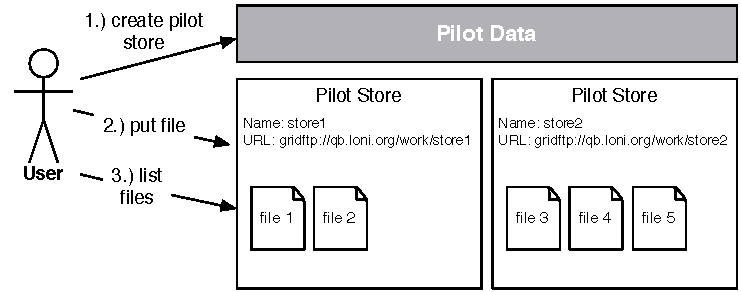
\includegraphics[width=0.8\textwidth]{figures/pilotstore.pdf}
    \caption{Pilot Data and Store Overview}
    \label{fig:figures_pilotstore}
\end{figure}

Pilot Data is a set of abstractions for expressing data localities and
affinities. Pilot Data can be used to create groups of file that are always used
together. This concept originates in
Filecules~\cite{Doraimani:2008:FGS:1383422.1383429} Pilot Data provides a set of
basic operations on top of these file groups Pilot Store: A container that
represents a logical group of physical files that share the same affinity.

Pilot Store Containers can be used to express data-data abstractions. 
Abstraction supports basic management tasks (create, delete, update,
move, list). 

\subsection{Overview}

The Pilot Data abstraction serves the following needs:
\begin{itemize}
	\item Reservation of physical disk space: acquisition of data storage (advanced reservation, place holder)
	\item Virtual destination: dynamically mapping of data to pilot stores.
	\item Runtime environment for $\alpha$ based data
	\item Automatic data partitioning and distribution
\end{itemize}


The pilot data abstraction provides two kinds of abstractions (see Figure~\ref{fig:figures_ps-instantiation}):
\begin{itemize}
    \item Pilot Data: Allows the logical grouping of files and the expression of data-data affinities. This collection of files can be associated with certain properties. One of this property is affinity.
    
    \item Pilot Store: Binds a pilot-data object to a actual physical resource. A pilot-store object can function as a placeholder object that reserves the space for a pilot-data object.
\end{itemize}


Figure~\ref{fig:figures_ps-instantiation} describes the differences between
pilot data object (abstract pilot stores) and pilot stores. A pilot data object
is a logical container and describes the properties of a group of files. A pilot
store is a placeholder reserving a certain amount of storage. By associating a
pilot data object to a pilot store the data is actually moved to the physically
location managed by the pilot store.

\begin{figure}[htbp]
    \centering
        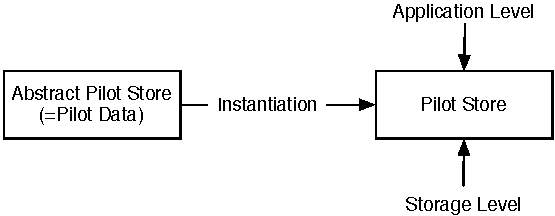
\includegraphics[width=0.6\textwidth]{figures/ps-instantiation.pdf}
    \caption{Level of Abstractions - Resource Binding}
    \label{fig:figures_ps-instantiation}
\end{figure}



	
\noindent	
Dynamic data:
\begin{itemize}
	\item Data to be generated (temporal)
	\item Data that is in place (spatial)
	\item Data that is changing (temporal)
	\item Data characteristics, properties
\end{itemize}	

\noindent
Analogies with Pilot-Job:
\begin{itemize}
	\item Assign pilot job to resource: $f^{1}(PJ_i) \rightarrow R_i$
	\item Assign task to pilot-job: $f^{2}(T_i) \rightarrow PJ_i$ 

	\item $g^{1} (D_i) \rightarrow PS_i$
	\item $g^{2} (PS_i) \rightarrow R_i$
\end{itemize}

\subsection{Pilot Data Architecture}


Data placement and locality is the key for a optimal performance of 
data-intensive applications. The Pilot Data Manager is responsible for 
optimizing the overall data distributions with respect to the application 
requirements. The architecture is designed as a \textbf{user-level overlay} on 
top of existing storage resources.

Figure~\ref{fig:figures_distributed_pilot_job} gives an overview of the
architecture. The system consists of two components: the pilot data manager and
the agents deployed on a specific physical storage resource. The manager is
responsible for 1) meta-data management, i.\,e.\ it keeps track of the pilot
stores that a pilot data object is associated with and 2) it schedules data
movements and data replications.

\begin{figure}[htbp]
    \centering
        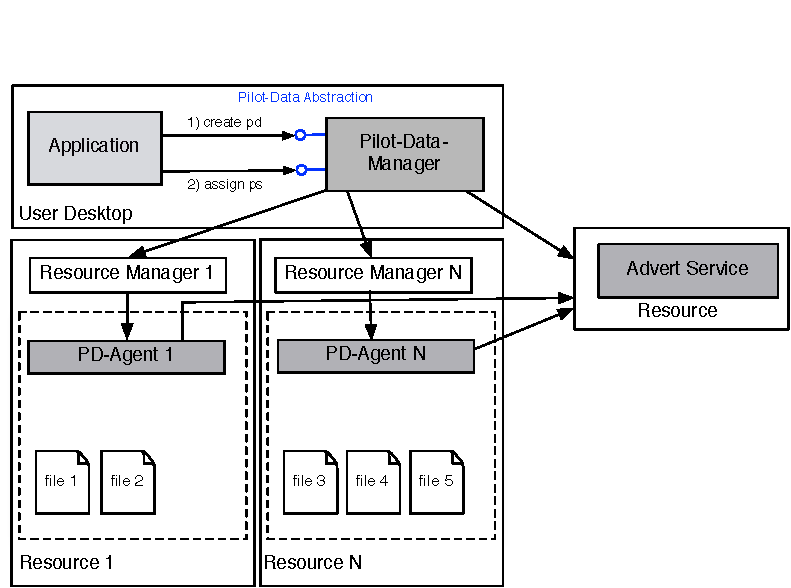
\includegraphics[height=3in]{figures/pilot-data-manager.pdf}
    \caption{Pilot Data Architecture}
    \label{fig:figures_distributed_pilot_job}
\end{figure}

Each pilot store is managed by an agent. The agent can be started manually or 
using the Pilot Data API. A possible implementation option would be the 
integration of the PD and BigJob agent, which is particularly useful for 
managing data-/compute-affinities.

A core part of the data manager is the data scheduler. The scheduler aims for a 
optimum of data and compute locality for an applications.
\begin{itemize}
	\item Move data to compute
	\item Move computer to data
	\item Streaming of data
	\item Data prefetching 
	\item Replication
\end{itemize}



\subsection{Data Movement}

The Pilot Data implementation is based on SAGA and thus, is infrastructure
independent. It supports all underlying SAGA adaptors (SSHFS, GridFTP) and
future adaptors such as Globus Online.

Work on optimizing file transfers: Kosar[2011]

Work on reliable file transfer: RFT, Globus Online

\subsection{Client API}

API for applications to distributively access data stored in pilot data groups.

\subsection{Related Work}

\subsubsection{iRods}


\subsubsection{Stork}


\subsubsection{BitDew}
\msnote{Interesting, didn't know it, does our group has experience with it?}

Random Notes
\begin{itemize}
	\item Focus on Desktop Grid
	\item Java-based implementation (ie difficult to interface with Python-based PS/SAGA)
	\item highly distributed: stable and volatile nodes
	\item pull model, i.e. a node pulls for new data
\end{itemize}


Mapping to BitDew:
\begin{itemize}
	\item Pilot Store in its current implementation covers Bitdew Data Catalog and Repository
	\item For data management and placement the Active Data API and the Bitdew data scheduler could be used
	\item Transfer Management is done via SAGA File API	
\end{itemize}

How to evolve pilot data/store?
\begin{itemize}
	\item Active management of data (e.g. replication, automatic affinity management) requires an active component:
	\begin{itemize}
		\item Manager/Agent model as in BigJob?
		\item Who runs active components? Started as part of batch job or separate install/start?
	\end{itemize}
\end{itemize}

Questions:
\begin{itemize}
    \item How should
    we store data in order to effectively cope with non-uniform demand for
    data? 
    \item How many copies of popular data objects do we need? 
    \item Where should we store them for effective load balancing?
\end{itemize}

\subsection{TODO/Future Work}
The current framework provides building blocks for expressing data localities and operation on file groups (similar to filecules).

Limitations:
\begin{itemize}
    \item No active agent that monitors state of files
    \item No placement policy support or autonomic behavior
    \item Infrastructures generally expose insufficient locality/topology information
    \item Compute – Data Affinity: Dynamic BigJob with affinity only provides a very coarse-grained affinity
    \item No policy for what’s happening if data is not available in right location:
    \begin{itemize}
        \item Run anyways – affinity is just an hint
    \end{itemize}
    \item When to move pilot stores? Move or copy?
    \item Move data to compute or visa versa?
    \item Data Replication: Identification of the same file: logical filename -> physical files. Manage replication process (consistency!)
\end{itemize}



\section{BFast Scenario for Dynamic Data}

According to this defined characteristics for data-intensive applications, BFAST can be classified as follows:
\begin{itemize}
    \item Data-Intensive: see ECLMS paper
    \item Compute-intensive: A significant amount of computing is required.
    \item Memory-intensive: The management of the memory is critical since BFAST 
    is doing a significant amount of computing on data in the main memory.
\end{itemize}


\textbf{Relationship to Dare}

Application-kernel: BFAST 
Application: Script that uses BFAST
Task: Instantiation of the kernel with a specific input and output





\textbf{Types of Input Files:}
\begin{itemize}
	\item static data: 
	\begin{itemize}
		\item reference genome
		\item index files
	\end{itemize}
	\item dynamic data: short-read files (ad-hoc generated depending on runtime)
\end{itemize}

\noindent
\textbf{Dynamic Scenarios:}
\begin{itemize}
	\item Moving generated short-read data to available resources. Transfer only 
	read file for resource 1 to resource 1.
	\begin{itemize}
	   \item group read files and transfer read files to vm. e.g. 4 read files for a 4 core VM
	   \item use replication?
	\end{itemize}
	
	\item Support processing of n experiments 

	\item re-partition of tasks to a larger number of available cores (dynamic 
	data that needs to re-generated as a consequence that there are new compute 
	elements available)
	\smnote{ As far as Bfast is concerned transferring the processed read files to a new resource is sufficient
	But if larger number of cores are available and we want to utilize them all we should stop the old read files and process the newly read files again. However, this would slow the time to completion.}
	
	

    \item Couple tasks to specific data elements
\end{itemize}

\section{BigJob API}
\label{sec:api}
\subsection{Resource Specification}


\begin{verbatim}
{
    "resource_url" : "pbspro://localhost/", 
    "number_nodes" : "2", 
    "processes_per_node":"4", 
    "allocation" : "loni_xyz", 
    "queue" : None, 
    "bigjob_agent": (BIGJOB_HOME + "/bigjob_agent_launcher.sh"), 
    "working_directory": (os.getcwd() + "/agent"), 
    "walltime":3600 
}
\end{verbatim}


\subsection{class: bigjob}


\begin{itemize}
	\item \_\_init\_\_
		\begin{itemize}
			\item database\_host
		\end{itemize}
	\item start\_pilot\_job
	\begin{itemize}
	   \item resource\_description\_dictionary
	\end{itemize}	
	\item get\_state	
	\item get\_state\_detail
	\item cancel
\end{itemize}

\subsection{class: subjob}
\begin{itemize}
\item \_\_init\_\_
		\begin{itemize}
			\item database\_host
		\end{itemize}
	\item submit\_job
	\begin{itemize}
		\item pilot\_url
		\item jd
	\end{itemize}

	\item get\_state

	\item delete\_job
\end{itemize}

\bibliographystyle{plain}
\bibliography{pilotjob,../../../Compiled_bibentries/saga.bib}
\end{document}
